\section{System Architecture}
\label{sec:system}

SMRITI is organized into twelve phases with strict boundary contracts:
each phase consumes only the immutable output artifact of the previous
phase and writes its own manifest recording every configuration parameter
used to produce its output. We describe the phases most relevant to this
paper's contributions; runtime governance, the dashboard, and the
evaluation layer's own internals are supporting infrastructure, not the
research contribution.

\begin{figure}[t]
  \centering
  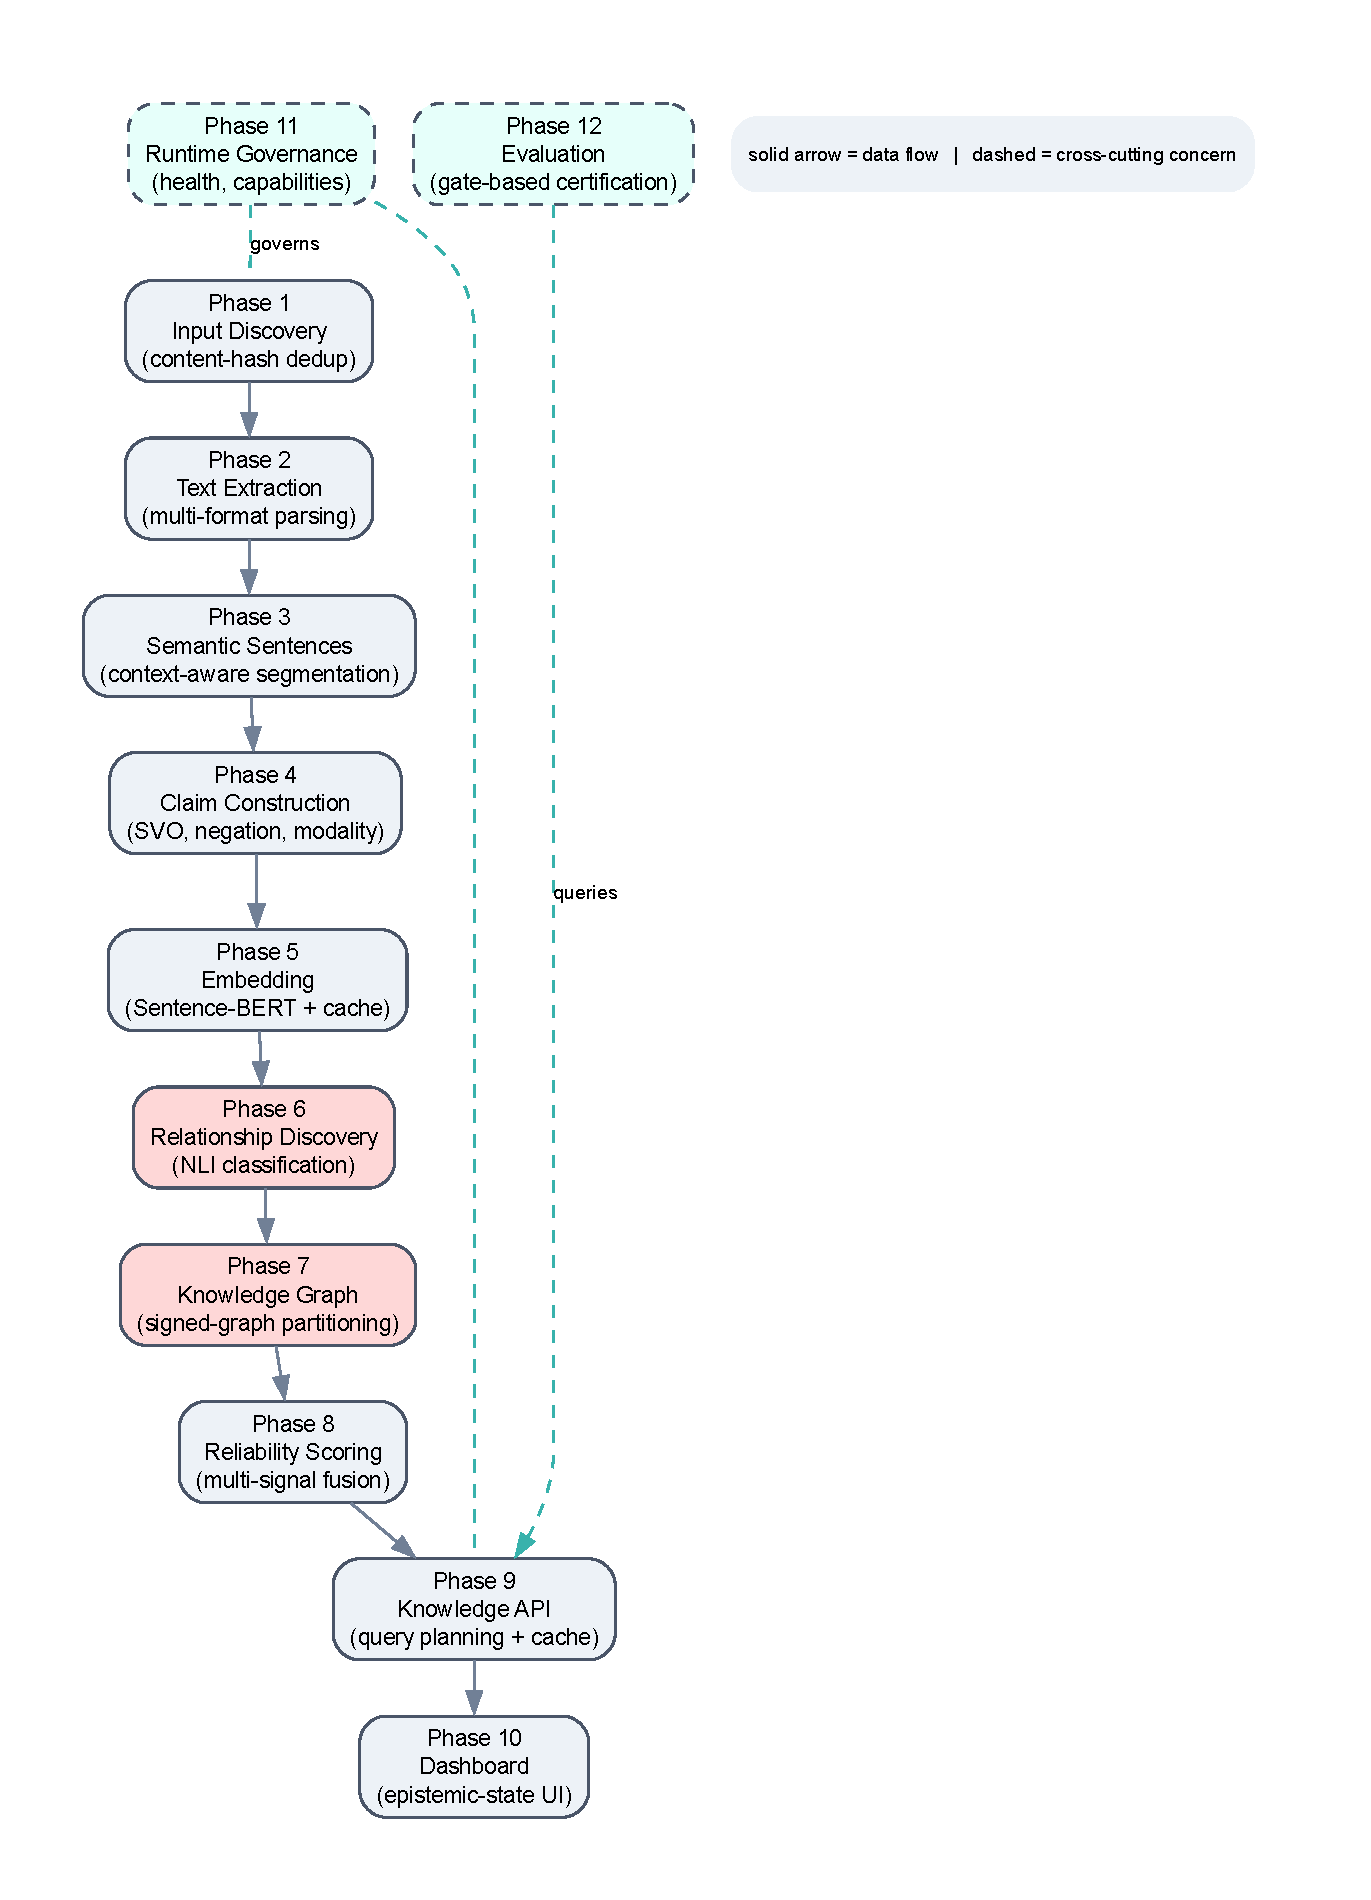
\includegraphics[width=\columnwidth]{figures/pipeline_architecture.pdf}
  \caption{SMRITI's twelve-phase pipeline. Phases 11 (runtime governance)
    and 12 (evaluation) are cross-cutting.}
  \label{fig:pipeline}
\end{figure}

\paragraph{Phases 1--4: from files to claims.} Phase 1 discovers input
files and deduplicates by content hash. Phase 2 extracts and normalizes
raw text. Phase 3 segments text into context-aware semantic sentences.
Phase 4 constructs claims via dependency-parse SVO extraction. \textbf{New
in this work}: immediately after Phase 3 and before claim construction, an
\emph{assertion-type classifier} categorizes every candidate sentence into
one of ten types (\texttt{DECLARATIVE\_ASSERTION}, \texttt{PROCEDURAL\_
INSTRUCTION}, \texttt{QUESTION}, \texttt{HEADING}, \texttt{METADATA},
\texttt{LIST\_ITEM}, \texttt{TABLE\_CELL}, \texttt{FRAGMENT}, \texttt{CODE},
\texttt{QUOTE}), using Phase 3's own block-type metadata plus lightweight
regex and dependency-structure rules --- no trained model. Only
\texttt{DECLARATIVE\_ASSERTION} proceeds to claim construction; every other
category is preserved losslessly in a \texttt{discarded\_candidates}
artifact rather than silently dropped. This directly targets the dominant
failure mode identified in this paper's predecessor: a large fraction of
``claims'' were bibliographic attribution lines, bare headings, and
ingredient-list fragments carrying no assertion at all.

\paragraph{Phases 5--6: embedding and relationship discovery.} Phase 5
embeds every claim with a cached Sentence-BERT model. Phase 6 retrieves
the top-$k$ nearest neighbors per claim by cosine similarity above a
threshold (exact search via FAISS's flat inner-product index, not
approximate), then classifies each candidate pair with a cross-encoder
NLI model into SUPPORTS / CONTRADICTS / REFINES / NEUTRAL.
\textbf{Rectified in this work}, in two parts:

\begin{enumerate}
  \item \emph{Arg-max resolution.} The resolver previously committed to
    CONTRADICTS whenever the contradiction score exceeded the entailment
    score by a margin, \emph{without ever checking the neutral score}. A
    pair with contradiction $=0.85$, entailment $=0.05$, but neutral
    $=0.90$ (neutral clearly the model's actual dominant class) still
    resolved to CONTRADICTS. The rule now requires the winning class to be
    the genuine arg-max of \{entailment, neutral, contradiction\}, beating
    \emph{both} alternatives by the configured margin; failing that, the
    pair falls through toward NEUTRAL or UNKNOWN (abstain --- never
    persisted to Phase 7).
  \item \emph{Relatedness gate.} A CONTRADICTS verdict additionally
    requires the two claims to share some detectable topical overlap
    (content-token Jaccard, boosted by any shared capitalized/entity-like
    token) --- a lightweight, model-free heuristic consistent with the
    resolver's own ``never calls an ML model'' design rule. This targets
    the specific population responsible for the original 100\% measured
    false-positive rate: candidate pairs that embedding retrieval surfaced
    as similar but that share no real subject matter.
\end{enumerate}

\paragraph{Phase 7: contradiction-safe graph construction.}
\label{sec:phase7}
No two claims connected by a CONTRADICTS edge may ever be assigned to the
same graph partition, even when they share a common SUPPORTS neighbor --- a
case that defeats the naive algorithm of deleting CONTRADICTS edges and
taking connected components (Figure~\ref{fig:partition}). SMRITI 2-colors
the contradiction-only subgraph via BFS and restricts union-find merging
along SUPPORTS/REFINES edges to same-colored nodes; components containing
an odd contradiction cycle are conservatively degraded into singleton
partitions. \S\ref{sec:bugs} describes a subtle correctness bug we found
and fixed in this exact code path.

\begin{figure}[t]
  \centering
  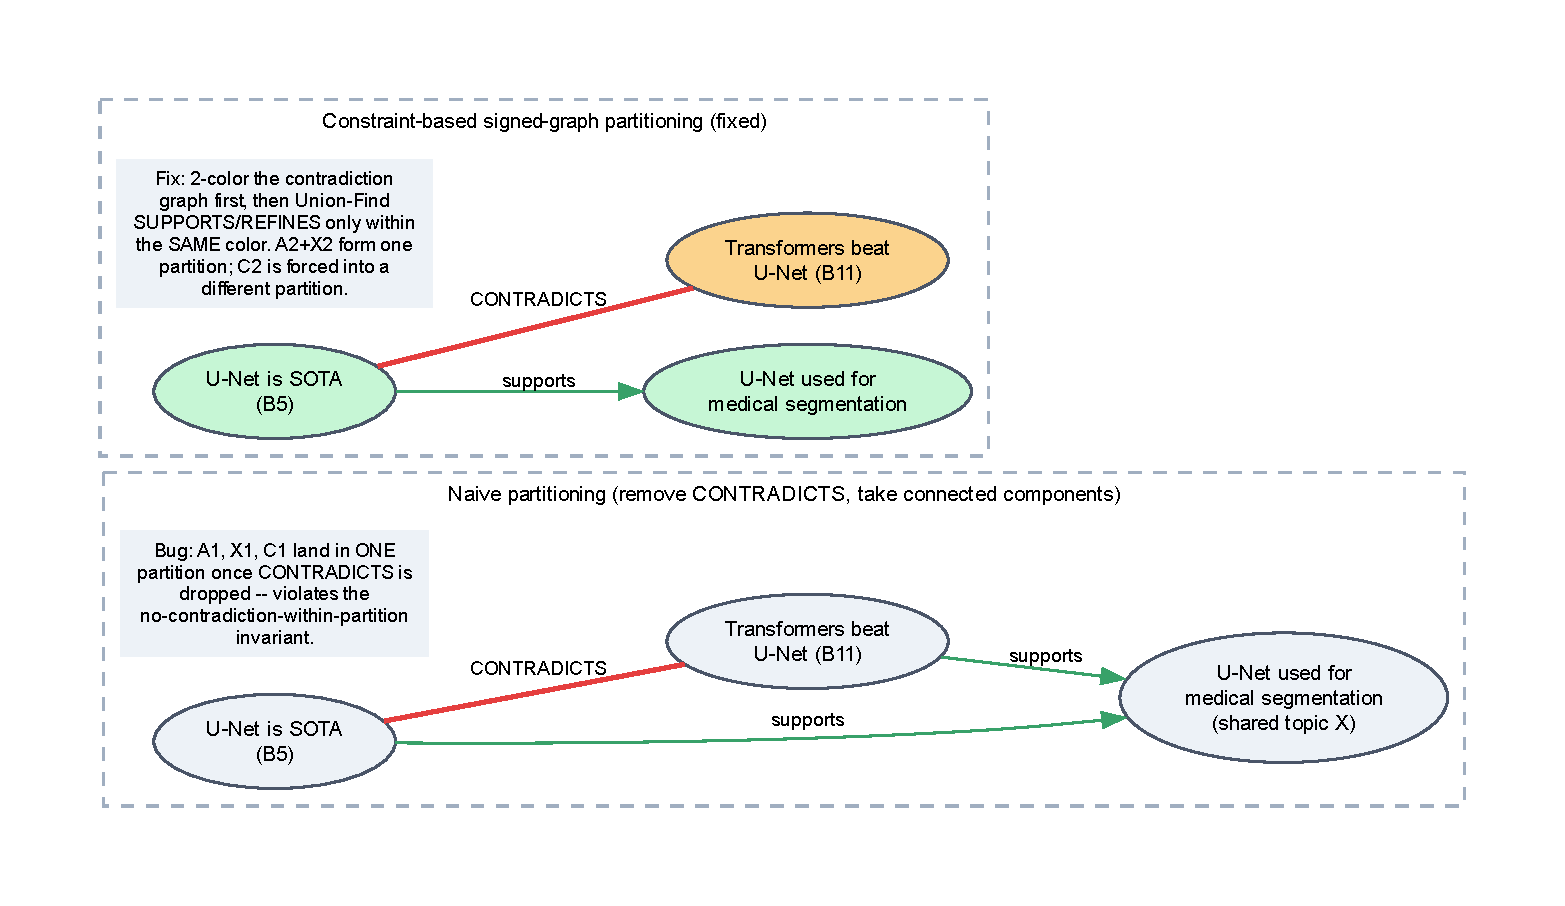
\includegraphics[width=\columnwidth]{figures/contradiction_partitioning.pdf}
  \caption{Naive vs.\ constraint-based partitioning when two contradicting
    claims share a supporting neighbor.}
  \label{fig:partition}
\end{figure}

\paragraph{Phase 8: evidence-aware reliability.} Independent signals
(evidence strength, evidence independence, source diversity, topology
strength, conflict pressure, temporal stability, completeness) are fused
into a single reliability index per claim, with a full decision record
(raw/constrained/final score, every constraint that fired) attached.
\textbf{Rectified in this work}, in two parts: (i) the evidence-independence
signal previously returned its \emph{maximum} value (1.0, ``fully
independent'') for a claim with zero supporting evidence at all ---
literally rewarding the absence of evidence. It now returns
\texttt{UNAVAILABLE} with value 0.0, withholding the positive contribution
a claim with nothing to evaluate was previously receiving. (ii)
\texttt{uncertainty\_score} is a metric reported alongside, but computed
separately from, \texttt{reliability\_index}; it previously combined only
evidence-sufficiency components (incompleteness, low diversity, low
independence) and never reflected \texttt{conflict\_pressure} at all, so a
claim under active, heavy dispute registered as less \emph{reliable} but
not more \emph{uncertain} --- two published numbers moving in a way its own
design does not intend. \texttt{conflict\_pressure} is now a fourth
weighted uncertainty component (\S\ref{sec:metamorphic} verifies this
directly via MR2). Both fixes are detailed in \S\ref{sec:bugs}.

\paragraph{Phases 9--12: API, dashboard, runtime, and evaluation.} Phase 9
exposes a query planner and cache. Phase 10 is an interactive dashboard
driven by claim epistemic state; it is a usability demonstration, not a
research contribution, and we do not discuss it further. Phase 11 provides
operational infrastructure (health monitoring, capability model, event
bus). Phase 12 is discussed at length in \S\ref{sec:cleanup}, since its
prior implementation is itself one of this paper's central findings.

\section{Scientific Cleanup of the Evaluation Layer}
\label{sec:cleanup}

The most consequential finding of this work is not an algorithmic bug --- it
is that the system's own self-evaluation layer (Phase 12) was, before this
paper, capable of producing a confident-looking numeric ``Scientific
Confidence Index'' (SCI) with no statistical meaning. Concretely, the prior
implementation:
\begin{itemize}
  \item computed a claim-extraction ``precision'' as
    $\mathrm{non\_empty\_claims} / \mathrm{total\_sampled}$ --- a
    non-emptiness check, not a semantic evaluation;
  \item invented a ``recall'' as $\min(1, \mathrm{total\_claims}/100)$,
    a formula with no relationship to any actual missed claim;
  \item hard-coded a ``generalization confidence'' of exactly 50.0 with the
    comment ``conservative --- single vault evaluation'', regardless of
    what was actually measured;
  \item computed ``statistical support'' as
    $\min(100, n_{\mathrm{experiments}} \times 15)$ --- a formula that
    rewards \emph{registering} more experiments, independent of whether any
    of them found anything;
  \item derived a Phase 7 ``partition purity'' from the number of
    partitions relative to claim count, with no reference to any
    independently-known partition label at all.
\end{itemize}
Every one of these is deleted, not patched. The replacement (frozen in
\texttt{evaluation/certification/claims.py}) is exactly five research
claims --- RC1 (claim extraction), RC2 (relationship resolution), RC3
(contradiction-safe partitioning), RC4 (evidence-aware reliability), RC5
(faithful explainability) --- each backed by exactly one experiment
(EXP-001..EXP-005) that either measures the claim against real,
independently-produced reference data, or reports a new
\texttt{NOT\_EVALUABLE} status with an explicit reason. \texttt{NOT\_
EVALUABLE} is distinct from both PASSED and FAILED: it means no real
measurement was possible, and it is never silently defaulted to a passing
numeric value. The Scientific Confidence Index field name is retained for
schema compatibility, but every sub-score it now reports is a real count or
ratio over real data (\S\ref{sec:results}); Gate 4 of the certification
report (``Statistical Verification'') blocks certification whenever this
honest number falls below threshold --- which, as of this paper, it does.

RC3 (contradiction-safe partitioning) is verified \emph{independently} of
Phase 7's own success: EXP-003 re-walks the live knowledge graph Phase 9
actually serves and checks, edge by edge, that no CONTRADICTS edge connects
two same-partition nodes, rather than trusting that Phase 7 would have
raised an exception on violation.
